\documentclass[12pt]{beamer} %Makes presentation
%\documentclass[handout]{beamer} %Makes Handouts
\usetheme{Singapore} %Gray with fade at top
\useoutertheme[subsection=false]{miniframes} %Supppress subsection in header
\useinnertheme{rectangles} %Itemize/Enumerate boxes
\usecolortheme{seagull} %Color theme
\usecolortheme{rose} %Inner color theme

\definecolor{light-gray}{gray}{0.75}
\definecolor{dark-gray}{gray}{0.55}
\setbeamercolor{item}{fg=light-gray}
\setbeamercolor{enumerate item}{fg=dark-gray}

\setbeamertemplate{navigation symbols}{}
\setbeamertemplate{mini frames}[default]
\setbeamercovered{dynamics}
\setbeamerfont*{title}{size=\Large,series=\bfseries}

%\setbeameroption{notes on second screen} %Dual-Screen Notes
%\setbeameroption{show only notes} %Notes Output

\newcommand{\heading}[1]{\noindent \textbf{#1}\\ \vspace{1em}}

\usepackage{bbding,color,multirow,times,ccaption,tabularx,graphicx,verbatim,booktabs,fixltx2e}
\usepackage{colortbl} %Table overlays
\usepackage[english]{babel}
\usepackage[latin1]{inputenc}
\usepackage[T1]{fontenc}

\title{212G: Does Public Opinion Matter?}

%\author[]{Thomas J. Leeper}
\institute[]{
  \inst{}%
  Department of Political Science and Government\\Aarhus University
}
\date[]{September 4, 2013}

\begin{document}

\frame{\titlepage}

\frame{\tableofcontents}

\section{Public Opinion?}
\frame{\tableofcontents[currentsection]}

\frame{
\heading{What comes to mind when you think of the term ``public opinion''?}
}

\section{Objectives and Exam}
\frame{\tableofcontents[currentsection]}

\frame{
\heading{Course Objectives}
\begin{enumerate}\itemsep1em
\item<1-> Explain what opinions are, how they are formed, and how they behave.
\item<2-> Apply knowledge of opinions and opinion measurement to the evaluation of survey public opinion research.
\item<3-> Explain different conceptualizations of political representation and their empirical implications.
\item<4-> Apply theories of representation to the evaluation of public processes and institutions.
\item<5-> Evaluate arguments about the proper role of public opinion in democracy and government.
\end{enumerate}
}

\frame{
\heading{Exam}
\begin{itemize}\itemsep1em
\item 7-day written ``take-home'' exam
\item 4,000 words
\item Answer two questions using relevant literature
\item Prepare using weekly writing activities
\item Date: not finalized yet, but probably week of Dec 9
\end{itemize}
}

\frame{
\heading{Weekly Activities}
\begin{itemize}\itemsep1em
\item Reading before class
\item Discussion
\item Short writing assignments
\item A ``preview'' lecture
\end{itemize}
}


\frame{
\heading{Proposal: Short assignments and discussion}
\begin{itemize}\itemsep1em
\item One student writes a one-page commentary
\item Another student writes a one-page response 
\item These are distributed 24 hours before class
\item Both students structure that week's discussion
\end{itemize}
}


\section{Outline for the course}
\frame{\tableofcontents[currentsection]}

\frame{
\heading{Outline}
\begin{itemize}\itemsep1em
\item What is public opinion? (4 weeks)
\item Effects on and of opinion (4 weeks)
\item Democratic implications (4 weeks)
\end{itemize}
}

\frame{
\heading{What is public opinion?}
\begin{itemize}\itemsep1em
\item Theory -- What is public opinion? (11 Sep)
\item Psychology I -- How do people form opinions? (18 Sep)
\item Psychology II -- Are opinions constrained? (2 Oct)
\item Methods -- How to measure opinion? (25 Sep)
\end{itemize}
}

\frame{
\heading{Effects on and of opinion}
\begin{itemize}\itemsep1em
\item Influences I -- What shapes public opinion(s)? (9 Oct)
\item Influences II -- Are opinions responsive? (23 Oct)
\item Participation I -- Do people act on their opinions? (30 Oct)
\item Participation II -- Do campaigns help citizens? (6 Nov)
\end{itemize}
}

\frame{
\heading{Democratic implications}
\begin{itemize}\itemsep1em
\item Aggregation -- From Micro to Macro? (13 Nov)
\item Representation I -- Public opinion matters? (20 Nov)
\item Representation II -- Groups matter? (27 Nov)
\item Opinion and Representation -- Theory and practice? (4 Dec)
\end{itemize}
}


\section{Introductions}
\frame{\tableofcontents[currentsection]}

\frame{
\heading{Introduce us to you}
\begin{itemize}
\item What is your name?
\item Where are you from?
\item What do you plan to do after AU?
\item What do you hope to learn in this class?
\end{itemize}
}

\frame<1-2>[label=me]{
\heading{Me}
\begin{itemize}
\item Name: Thomas Leeper
\item<2-> From: Shoreview, Minnesota, United States
\item<3-> Plans: I plan to teach and research in the US
\item<4-> Learn: How to get all of you engaged in this course \& What your perspectives are on the public opinion and its role in contemporary democracy
\end{itemize}
}

\frame{
\heading{Me}
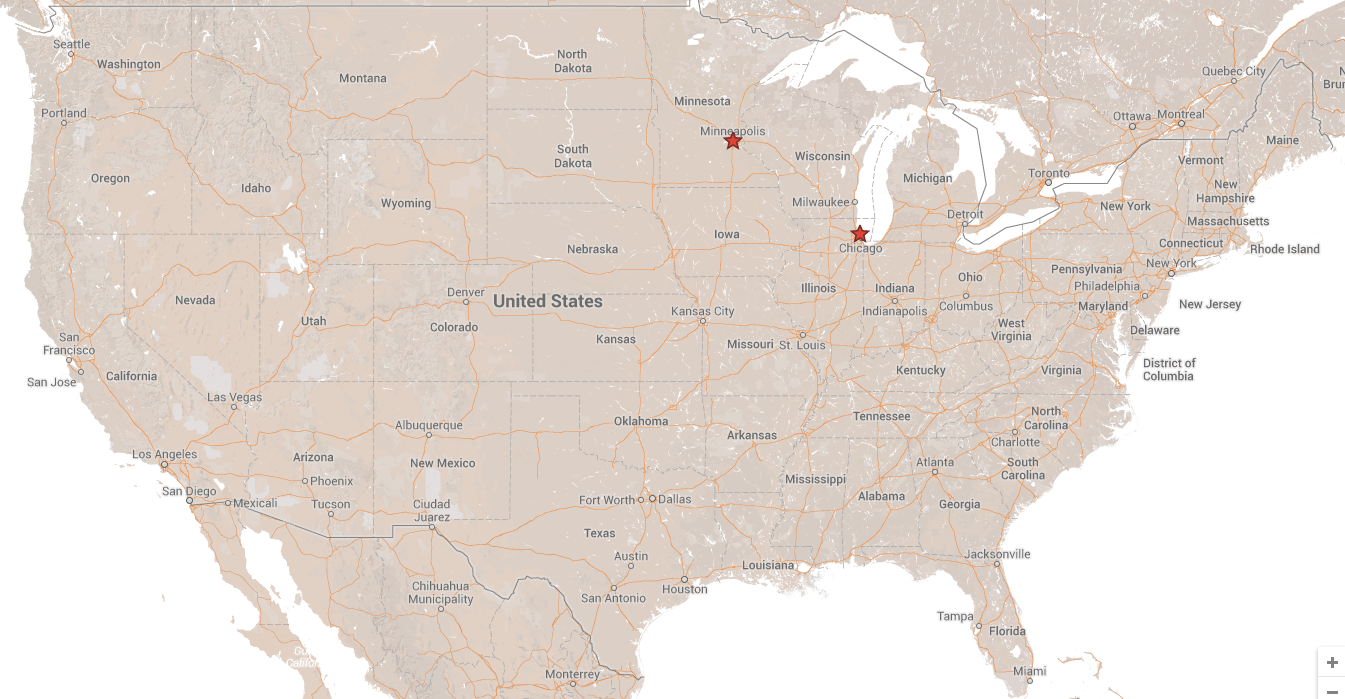
\includegraphics[width=\textwidth]{UnitedStates}
}

\againframe<3-4>{me}

\frame{
\heading{Form groups and introduce yourselves for 2--3 minutes}
}


\appendix
\frame{}

\end{document}
